\documentclass[12pt,a4paper]{report}
\usepackage[utf8]{inputenc}
\usepackage{array,geometry,graphicx,fancyhdr,amsmath,amsfonts,amssymb,color,hyperref,listings}
\usepackage{booktabs,multirow,subcaption,titlesec,multicol,caption,colortbl,enumitem}

% ===================== PROFESSIONAL COLOR SCHEME =====================
% Define professional color palette
\definecolor{primaryblue}{RGB}{0,82,165}        % Deep professional blue
\definecolor{secondaryblue}{RGB}{25,118,210}    % Medium blue 
\definecolor{accentblue}{RGB}{100,181,246}      % Light blue accent
\definecolor{lightblue}{RGB}{173,216,230}       % Light blue for backgrounds
\definecolor{darkgray}{RGB}{66,66,66}           % Professional dark gray
\definecolor{mediumgray}{RGB}{117,117,117}      % Medium gray
\definecolor{lightgray}{RGB}{238,238,238}       % Light gray for backgrounds

% Table color definitions
\definecolor{tableheader}{RGB}{0,82,165}         % Primary blue for headers
\definecolor{tablebody}{RGB}{240,248,255}        % Very light blue
\definecolor{tableaccent}{RGB}{25,118,210}       % Secondary blue accent
\definecolor{tableborder}{RGB}{0,82,165}         % Primary blue border
\definecolor{headertext}{RGB}{255,255,255}       % White text for headers
\definecolor{bodytext}{RGB}{66,66,66}            % Dark gray text
\definecolor{tablealt1}{RGB}{248,251,255}        % Alternating row color 1
\definecolor{tablealt2}{RGB}{235,245,251}        % Alternating row color 2

% Subtle highlight colors
\definecolor{techcolor}{RGB}{41,128,185}         % Subtle blue for technologies
\definecolor{companycolor}{RGB}{156,39,176}      % Subtle purple for company names
\definecolor{projectcolor}{RGB}{142,68,173}      % Subtle purple for project names
\definecolor{skillcolor}{RGB}{211,84,0}          % Orange for skills/features
\definecolor{toolcolor}{RGB}{52,152,219}         % Light blue for tools
\definecolor{featurecolor}{RGB}{230,126,34}      % Orange for features/highlights
\definecolor{impactcolor}{RGB}{192,57,43}        % Deep red for business impact

% Table styling commands
\newcommand{\tableheaderrow}{\rowcolor{tableheader}}
\newcommand{\tablealtrow}{\rowcolor{tablealt1}}
\newcommand{\tablealtrowtwo}{\rowcolor{tablealt2}}
\setlength{\arrayrulewidth}{1.2pt}

% Highlight macros
\newcommand{\tech}[1]{\textcolor{techcolor}{\textbf{#1}}}
\newcommand{\company}[1]{\textcolor{companycolor}{\textbf{#1}}}
\newcommand{\project}[1]{\textcolor{projectcolor}{\textbf{#1}}}
\newcommand{\skill}[1]{\textcolor{skillcolor}{\textbf{#1}}}
\newcommand{\tool}[1]{\textcolor{toolcolor}{\textbf{#1}}}
\newcommand{\feature}[1]{\textcolor{featurecolor}{\textbf{#1}}}
\newcommand{\impact}[1]{\textcolor{impactcolor}{\textbf{#1}}}

% Custom citation color
\let\oldcite\cite
\renewcommand{\cite}[1]{\textcolor{impactcolor}{\oldcite{#1}}}

% Colored itemize environments
\newenvironment{coloritemize}
{\begin{itemize}[label=\textcolor{primaryblue}{$\bullet$}]}
{\end{itemize}}
\newenvironment{techitemize}
{\begin{itemize}[label=\textcolor{techcolor}{$\blacksquare$}]}
{\end{itemize}}
\newenvironment{projectitemize}
{\begin{itemize}[label=\textcolor{projectcolor}{$\diamond$}]}
{\end{itemize}}

% Caption styling
\captionsetup{
    font={bf,small},
    textfont={color=bodytext},
    labelfont={color=primaryblue, bf},
    justification=centering,
    singlelinecheck=false,
    labelsep=period,
    skip=10pt,
    position=bottom
}
\captionsetup[sub]{
    font={bf,footnotesize},
    textfont={color=bodytext},
    labelfont={color=secondaryblue, bf},
    justification=centering,
    singlelinecheck=false,
    labelsep=period,
    skip=8pt
}

% Hyperref colors
\hypersetup{
    colorlinks=true,
    linkcolor=primaryblue,
    filecolor=secondaryblue,      
    urlcolor=accentblue,
    pdftitle={Industrial Attachment Report},
    pdfauthor={Sajidur Rahman Tarafder},
    pdfsubject={Industrial Attachment Report - Netro Systems}
}

% Code listings styling
\lstset{
    basicstyle=\ttfamily\footnotesize,
    backgroundcolor=\color{lightgray},
    frame=leftline,
    framerule=3pt,
    rulecolor=\color{primaryblue},
    breaklines=true,
    captionpos=b,
    numbers=left,
    numberstyle=\tiny\color{darkgray}\bfseries,
    stepnumber=1,
    numbersep=12pt,
    keywordstyle=\color{primaryblue}\bfseries,
    commentstyle=\color{mediumgray}\itshape,
    stringstyle=\color{secondaryblue},
    emphstyle=\color{accentblue}\bfseries,
    showstringspaces=false,
    tabsize=2,
    xleftmargin=20pt,
    framexleftmargin=15pt
}

% Chapter, section formatting
\titleformat{\chapter}[display]
  {\normalfont\huge\bfseries\color{primaryblue}}
  {\colorbox{primaryblue}{\textcolor{white}{\chaptertitlename\ \thechapter}}}{20pt}
  {\Huge\color{primaryblue}}
  [\vspace{5pt}{\centering\color{primaryblue}\titlerule[2pt]}]
\titlespacing*{\chapter}{0pt}{50pt}{40pt}

\titleformat{\section}[hang]
  {\normalfont\Large\bfseries\color{primaryblue}}
  {\colorbox{primaryblue}{\textcolor{white}{\makebox[2em]{\thesection}}}}{0.5em}
  {\color{primaryblue}}
  [\vspace{3pt}{\color{primaryblue}\titlerule[1.5pt]}]
\titlespacing*{\section}{0pt}{3.5ex plus 1ex minus .2ex}{2.3ex plus .2ex}

\titleformat{\subsection}[hang]
  {\normalfont\large\bfseries\color{secondaryblue}}
  {\colorbox{secondaryblue}{\textcolor{white}{\makebox[2.5em]{\thesubsection}}}}{0.5em}
  {\color{secondaryblue}}
  [\vspace{2pt}{\color{secondaryblue}\titlerule[1pt]}]
\titlespacing*{\subsection}{0pt}{3.25ex plus 1ex minus .2ex}{1.5ex plus .2ex}

\titleformat{\subsubsection}[hang]
  {\normalfont\normalsize\bfseries\color{accentblue}}
  {\colorbox{accentblue}{\textcolor{white}{\makebox[3em]{\thesubsubsection}}}}{0.5em}
  {\color{accentblue}}
  [\vspace{1pt}{\color{accentblue}\titlerule[0.8pt]}]
\titlespacing*{\subsubsection}{0pt}{3.25ex plus 1ex minus .2ex}{1.5ex plus .2ex}

% Custom titlepage formatting
\geometry{
    a4paper,
    left=2.5cm,
    right=2.5cm,
    top=2.5cm,
    bottom=2.5cm,
    headheight=15pt,
    headsep=20pt,
    footskip=20pt,
    includeheadfoot
}
\pagestyle{fancy}
\fancyhf{}
\fancyhead[L]{\textcolor{primaryblue}{\textbf{Industrial Attachment Report}}}
\fancyhead[R]{\textcolor{primaryblue}{\textbf{Netro Systems Limited}}}
\fancyfoot[C]{\textcolor{primaryblue}{\textbf{\thepage}}}
\renewcommand{\contentsname}{\textcolor{primaryblue}{Table of Contents}}
\renewcommand{\headrulewidth}{2pt}
\renewcommand{\footrulewidth}{1pt}
\renewcommand{\headrule}{\hbox to\headwidth{%
    \color{primaryblue}\leaders\hrule height \headrulewidth\hfill}}
\renewcommand{\footrule}{\hbox to\headwidth{%
    \color{lightgray}\leaders\hrule height \footrulewidth\hfill}}

% Redefine plain page style to use primary blue page numbers
\fancypagestyle{plain}{%
    \fancyhf{}%
    \fancyfoot[C]{\textcolor{primaryblue}{\textbf{\thepage}}}%
    \renewcommand{\headrulewidth}{0pt}%
    \renewcommand{\footrulewidth}{0pt}%
}

\begin{document}

\begin{titlepage}
    \thispagestyle{empty}
    \centering

    % University motto with elegant styling
    {\large \textit{\textbf{\textcolor{darkgray}{Heaven's Light is Our Guide}}}}\\[0.4cm]

    % University logo
    \includegraphics[width=4.5cm]{ruet_logo.png} \\[0.4cm]

    % Department and University
    {\Large \textcolor{secondaryblue}{\textbf{Department of Computer Science \& Engineering}}}\\[0.3cm]
    {\Large \textcolor{primaryblue}{\textbf{Rajshahi University of Engineering \& Technology}}}\\[1.8cm]

    % Report title
    {\Huge \textcolor{primaryblue}{\textbf{Industrial Attachment Report}}}\\[0.8cm]
    {\LARGE \textcolor{skillcolor}{\textbf{Netro Systems Limited}}}\\[2cm]

    % Student and supervisor info
    \begin{minipage}{0.45\textwidth}
        \raggedright
        {\Large \textcolor{primaryblue}{\textbf{Submitted by:}}}\\[0.3cm]
        {\large \textbf{Sajidur Rahman Tarafder}}\\
        \vspace{0.2cm}
        {\large \textbf{Roll: 2003154}}\\
        \vspace{0.2cm}
        {\large \textbf{Section: C}}\\
        \vspace{0.2cm}
        {\large \textbf{Session: 2020-21}}\\
        \vspace{0.2cm}
        {\large \textbf{Dept of CSE, RUET}}\\
    \end{minipage}%
    \hfill%
    \begin{minipage}{0.45\textwidth}
        \raggedleft
        {\Large \textcolor{primaryblue}{\textbf{Academic Supervisor:}}}\\[0.3cm]
        {\large \textbf{A.F.M. Minhazur Rahman}}\\
        {\large \textbf{Assistant Professor}}\\
        {\large \textbf{Dept. of CSE, RUET}}\\[0.8cm]

    {\Large \textcolor{primaryblue}{\textbf{Industrial Supervisor:}}}\\[0.3cm]
    {\large \textbf{Md. Raihanul Islam}}\\
    {\large \textbf{HR Manager}}\\
    {\large \textbf{Netro Systems Limited}}\\
    \end{minipage}

    \vfill
\end{titlepage}

\chapter*{\textcolor{primaryblue}{Declaration}}
\addcontentsline{toc}{chapter}{Declaration}

I, \textcolor{skillcolor}{\textbf{Sajidur Rahman Tarafder}}, hereby declare that this report on the industrial attachment completed at \textcolor{companycolor}{\textbf{Netro Systems Limited}} is my original work. All information and descriptions provided in this report are based on my own observations and experience during the attachment period. I have not used any sources beyond those permitted by academic integrity, and I acknowledge all contributions and assistance from others. This report has not been submitted for any other degree or academic award in any institution.

\vspace{1cm}

\noindent
\textcolor{darkgray}{\textbf{Sajidur Rahman Tarafder}}\\
\textcolor{darkgray}{Roll: 2003154}\\
\textcolor{darkgray}{Department of Computer Science \& Engineering}\\
\textcolor{darkgray}{Rajshahi University of Engineering \& Technology}

\chapter*{\textcolor{primaryblue}{Acknowledgment}}
\addcontentsline{toc}{chapter}{Acknowledgment}

I am grateful to the \textcolor{companycolor}{\textbf{Department of CSE, RUET}}, for facilitating this industrial attachment. I would like to thank my academic supervisor, \textcolor{skillcolor}{\textbf{A.F.M. Minhazur Rahman}}, for guidance and support throughout the preparation of this report.

My special thanks go to \textcolor{companycolor}{\textbf{Netro Systems Limited}} for providing me with the opportunity to gain practical experience in a professional environment. In particular, I would like to thank \textcolor{skillcolor}{\textbf{Md. Raihanul Islam}}, the Human Resources Manager at Netro Systems, for coordinating the attachment program and supporting my learning. I am also grateful to the mentors and all colleagues at Netro Systems for introducing me to their workflows and technologies. Their guidance and patience greatly enriched my learning experience.

Special recognition goes to the development team members who provided valuable insights into modern software development practices and the management team for creating a conducive learning environment.

Finally, I would like to thank my family and friends for their unwavering support during this period.

\chapter*{\textcolor{primaryblue}{Executive Summary}}
\addcontentsline{toc}{chapter}{Executive Summary}

This report documents a 10-day industrial attachment undertaken in a student team at \textcolor{companycolor}{\textbf{Netro Systems Limited}} from March 9, 2025, to March 20, 2025. The attachment aimed to integrate theoretical knowledge from my Computer Science and Engineering program with practical experience in a professional software development environment. During this period, we began with orientation sessions covering the company’s culture, services, and development processes. We were introduced to Agile \cite{ref8} methodologies and used Kanban boards to manage tasks within cross-functional teams. 

I contributed to a major project called \textcolor{projectcolor}{\textbf{\textit{Smart Pathshala}}}, a school management system, by assisting the development team with design, testing, and documentation tasks while adhering to credential access limitations. I also supported various development activities such as reviewing user interface designs, understanding backend API integration, and performing module-level testing. The work involved technologies like React \cite{ref3}, Node.js \cite{ref5}, and MongoDB for data storage. Over the course of the attachment, we participated in daily stand-up meetings, used Git for version control, and regularly presented progress updates to our mentors.


Through this attachment, I observed the organizational structure and operational processes of Netro Systems. Chapter 2 describes the company's history, mission, departments, and core services, including its emphasis on quality and a collaborative work culture. Chapter 3 provides a detailed overview of the Smart Pathshala project, covering the problem analysis, literature background, and development methodology. Chapter 4 outlines the tools and techniques used, such as development frameworks, version control, and testing tools. Chapters 5 and 6 discuss societal, safety, and ethical considerations encountered during the attachment, including workplace health measures, data privacy practices, and cultural awareness in design. Chapter 7 reflects on the technical and soft skills I gained, while Chapter 8 details the challenges I faced and the lessons learned. Chapter 9 summarizes my specific contributions to the organization, and Chapter 10 concludes with recommendations for the company, the university, and future interns.

Overall, the industrial attachment provided valuable hands-on experience in software engineering \cite{ref11}. I developed new technical competencies, improved problem-solving abilities, and gained insight into the professional responsibilities of an engineer. The recommendations and reflections in this report are intended to contribute to continuous improvement for all stakeholders involved in industrial training.

\tableofcontents
\listoftables
\listoffigures

\chapter*{\textcolor{primaryblue}{List of Abbreviations}}
\addcontentsline{toc}{chapter}{List of Abbreviations}

\begin{table}[h!]
\centering
\begin{tabular}{p{3cm} p{10cm}}
\toprule
\textcolor{primaryblue}{\textbf{Abbreviation}} & \textcolor{primaryblue}{\textbf{Full Form}} \\
\midrule
\textcolor{darkgray}{API} & Application Programming Interface\\
\textcolor{darkgray}{CSE} & Computer Science \& Engineering\\
\textcolor{darkgray}{MVC} & Model-View-Controller\\
\textcolor{darkgray}{UI} & User Interface\\
\textcolor{darkgray}{UX} & User Experience\\
\textcolor{darkgray}{SaaS} & Software as a Service\\
\textcolor{darkgray}{IDE} & Integrated Development Environment\\
\textcolor{darkgray}{CI/CD} & Continuous Integration/Continuous Deployment\\
\textcolor{darkgray}{NDAs} & Non-Disclosure Agreements\\
\textcolor{darkgray}{QA} & Quality Assurance\\
\textcolor{darkgray}{RUET} & Rajshahi University of Engineering \& Technology\\
\textcolor{darkgray}{PHP} & Hypertext Preprocessor\\
\textcolor{darkgray}{JEST} & JavaScript Testing Framework\\
\textcolor{darkgray}{AWS} & Amazon Web Services\\
\textcolor{darkgray}{JSON} & JavaScript Object Notation\\
\bottomrule
\end{tabular}
\end{table}

\chapter{Introduction}
\section{Background of Industrial Attachment}
Industrial attachment (internship) is a mandatory component of the engineering curriculum at RUET. It bridges classroom learning and industry practice by exposing students to real-world engineering projects. Netro Systems Limited was selected for my internship due to its cutting-edge work in software development and diversified portfolio. The attachment provided an opportunity to apply theoretical knowledge to practical problems, understand professional work environments, and fulfill degree requirements.

\section{Importance in Achieving Engineering Program Outcomes}
The attachment helped me bridge academic knowledge with industry practice. At Netro,
I observed how teams design and deliver end-to-end software solutions, including UI/UX
design, SaaS platforms, and AI-driven applications. The hands-on experience ensured that skills such as software design, coding, and testing were practiced to industry standards.Also observing an management system project allowed me to apply data-driven
problem-solving and core engineering principles to a practical task. 

\section{Objectives of the Attachment}
The primary objectives of this attachment were:
\begin{coloritemize}
    \item To gain practical experience in a professional software development setting.
    \item To contribute to a real project (Smart Pathshala) and implement technical solutions.
    \item To learn and apply software engineering \cite{ref11} tools and practices used at Netro Systems.
    \item To enhance understanding of the software development lifecycle, teamwork, and communication.
    \item To develop soft skills such as problem-solving, adaptability, and professional responsibility.
\end{coloritemize}

\section{Scope and Limitations}
The attachment focused on software development tasks within the Smart Pathshala project. Scope included backend and frontend development, database design, and user interface implementation. Due to time constraints (10 days), I did not engage in
long-term tasks like deployment or system maintenance. My role was mainly supportive,
but I still gained a broad overview of full-stack development

\section{Methodology}
The project followed an Agile \cite{ref8} Development methodology with iterative sprints. I participated in requirement analysis meetings and helped create user stories and prototypes using Figma. Two-week sprint cycles were employed: each cycle involved planning, development, testing, and review. Version control (Git) and code reviews maintained quality. I also performed continuous self-study (reading documentation, online tutorials) to learn new tools as needed. Methodologies for software design (MVC architecture) and testing (unit and integration tests) were used to ensure a systematic approach.

\section{Structure of the Report}
\label{sec:report_structure}
To guide readers through the ensuing chapters, this section outlines how the report is organized. Each chapter focuses on a distinct aspect of the industrial attachment and collectively provides a comprehensive narrative:
\begin{coloritemize}
    \item \impact{\textbf{Chapter 1: Introduction}} – Presents the background, importance, objectives, scope, methodology, and structure of the report.
    \item \impact{\textbf{Chapter 2: Organization Overview}} – Profiles \company{Netro Systems Limited}, including its mission, vision, values, organizational structure, market presence, and growth metrics.
    \item \impact{\textbf{Chapter 3: Project Overview}} – Describes the \project{Smart Pathshala} project, detailing problem analysis, literature background, system design, and features implemented during the attachment.
    \newpage
    \item \impact{\textbf{Chapter 4: Tools and Techniques}} – Summarizes the key technologies, frameworks, and tools used throughout the attachment, such as React, Node.js, MongoDB, version control, and testing tools.
    \item \impact{\textbf{Chapter 5: Societal, Health, Safety, Legal & Cultural Considerations}} – Discusses health, safety, and societal implications encountered in the workplace and project, including workplace ergonomics and data privacy.
    \item \impact{\textbf{Chapter 6:  Professional Ethics & Responsibilities}} – Explores ethical issues such as confidentiality, intellectual property, and professional conduct within the context of the internship.
    \item \impact{\textbf{Chapter 7: Skills Gained & Lifelong Learning}} – Reflects on the technical and soft skills developed during the attachment, encompassing coding competencies, teamwork, communication, and problem‑solving.
    \item \impact{\textbf{Chapter 8: Challenges & Solutions}} – Describes the obstacles faced, strategies employed to overcome them, and the lessons drawn from those experiences.
    \item \impact{\textbf{Chapter 9: Contributions to the Organization}} – Summarizes the specific contributions made to Netro Systems and to the \project{Smart Pathshala} project, highlighting deliverables and impact.
    \item \impact{\textbf{Chapter 10: Conclusion and Recommendations}} – Concludes the report with key takeaways and provides recommendations for the company, the university, and future interns.
\end{coloritemize}

\chapter{Organization Overview}
\section{Company Profile and Global Presence}
\company{Netro Systems Limited}, also known as Netro Creative, is a software company based in
Rajshahi, Bangladesh \cite{ref1}. The company specializes in web and mobile application develop-
ment, UI/UX design, and SaaS solutions. It provides end-to-end software services for
startups, SMEs, and enterprises, focusing on high-quality, scalable, and user-friendly ap-
plications. Netro’s team consists of developers, designers, and project managers who
follow modern software engineering \cite{ref11} practices, including Agile \cite{ref8} Scrum

\subsection{Corporate Headquarters and Locations}
\begin{coloritemize}
    \item \impact{Primary Headquarters:} Level 6B, Silicon Tower, Hi-Tech Park, Rajshahi, Bangladesh
    \item \impact{International Office:} Preston, Lancashire, United Kingdom
    \item \impact{Operational Focus:} Global software development with emphasis on Education, Finance, Telecommunication, Healthcare, Logistics, and eCommerce industries
\end{coloritemize}

\begin{figure}[h!]
\centering
    
\includegraphics[width=0.3\textwidth]{Figures/logo.png}
    \caption{Logo of Netro Systems}
\end{figure}


\section{Mission, Vision, and Core Values}
\subsection{Mission Statement}
Netro Systems' mission is to \textbf{empower businesses through innovative digital solutions} that drive growth, enhance efficiency, and create meaningful user experiences. The company is dedicated to transforming complex business challenges into elegant, scalable software solutions that deliver measurable value to clients and their end-users.

\subsection{Vision Statement}
To become the \textbf{leading global software development partner} recognized for delivering exceptional digital experiences that shape the future of technology and business innovation.

\subsection{Core Values}
\begin{coloritemize}
    \item \skill{Innovation Excellence:} Continuously pushing the boundaries of technology to deliver cutting-edge solutions
    \item \skill{Client-Centric Approach:} Placing client success at the center of every decision and development process
    \item \skill{Quality Commitment:} Maintaining the highest standards in software development, design, and delivery
    \item \skill{Collaborative Culture:} Foster teamwork, knowledge sharing, and collective problem-solving
    \item \skill{Ethical Practices:} Operating with integrity, transparency, and respect for all stakeholders
    \item \skill{Continuous Learning:} Embracing new technologies and methodologies to stay ahead of industry trends
\end{coloritemize}

\section{Company Growth and Market Position}
From its humble beginnings as a boutique software development firm, Netro Systems has evolved into a globally recognized technology partner within just 5 years of operation. The company has achieved remarkable growth milestones:

\begin{table}[h!]
\centering
\caption{Netro Systems Growth Metrics and Achievements}
\label{tab:growth_metrics}
\begin{tabular}{p{6cm} p{3cm} p{6cm}}
\toprule
\rowcolor{tableheader}\textcolor{headertext}{\textbf{Metric}} & \textcolor{headertext}{\textbf{Achievement}} & \textcolor{headertext}{\textbf{Business Impact}} \\
\midrule
\tablealtrow \impact{Global Clients Served} & \textbf{230+ Projects} & Successfully delivered across North America, Europe, and Asia \\
\impact{Client Satisfaction Rate} & \textbf{119+ Satisfied Clients} & Rated 5.0 on Clutch, 4.5 on GoodFirms, and 5.0 on Trustpilot \\
\tablealtrow \impact{Client Funding Raised} & \textbf{\$70M+ Total} & Netro-built MVPs helped clients secure substantial funding \\
\impact{User Engagement Growth} & \textbf{6x Increase} & Average user engagement improvement after UX revamps \\
\tablealtrow \impact{Mobile App Adoption} & \textbf{8x Growth} & User base expansion within first month post-launch \\
\impact{International Brands} & \textbf{200+ Brands} & Diverse portfolio across multiple industries and regions \\
\bottomrule
\end{tabular}
\end{table}

\newpage
\subsection{Global Market Presence and Key Achievements}

\begin{table}[h!]
\centering
\caption{Netro Systems Global Market Presence}
\label{tab:global_presence}
\begin{tabular}{p{6cm} p{8cm}}
\toprule
\tableheaderrow \textcolor{headertext}{\textbf{Region}} & \textcolor{headertext}{\textbf{Market Coverage}} \\
\midrule
\tablealtrow \impact{North America} & USA clients with focus on enterprise solutions and startups \\
\impact{Europe} & UK and Germany operations, serving fintech and ecommerce sectors \\
\tablealtrow \impact{Asia} & Bangladesh headquarters, Singapore partnerships for regional expansion \\
\impact{Middle East} & Oman presence expanding into Gulf Cooperation Council markets \\
\bottomrule
\end{tabular}
\end{table}

\newpage
\section{Organizational Structure and Leadership}
Netro Systems employs a modern, collaborative organizational structure designed to foster innovation, efficiency, and cross-functional teamwork. The company maintains a relatively flat hierarchy that encourages open communication and rapid decision-making while ensuring clear accountability and leadership.

\subsection{Executive Leadership Team}
Netro Systems operates under visionary leadership that guides the company's technological evolution and international growth:

\begin{table}[h!]
\centering
\caption{Netro Systems Executive Leadership Structure}
\label{tab:leadership}
\begin{tabular}{p{3cm} p{3.5cm} p{7.5cm}}
\toprule
\tableheaderrow \textcolor{headertext}{\textbf{Position}} & \textcolor{headertext}{\textbf{Name}} & \textcolor{headertext}{\textbf{Key Responsibilities}} \\
\midrule
\tablealtrow \impact{CEO} & \textbf{Asiq Mohammed} & Visionary leader with experience in product innovation, responsible for overall company strategy, client relations, and international growth \\
\impact{CTO} & \textbf{Ahamed Lincon} & Leads technical innovation, product development, AI integrations, and ensures technical excellence across all projects \\
\tablealtrow \impact{COO} & \textbf{Sultan M.} & Manages operational processes, project timelines, quality assurance, and resource allocation for optimal efficiency \\
\impact{CMO} & \textbf{Altamira Tripty} & Oversees branding strategies, communications, digital marketing initiatives, and global market expansion \\
\tablealtrow \impact{HR} & \textbf{Raihanul Islam} & Responsible for talent acquisition, corporate relations, organizational culture, and business development \\
\bottomrule
\end{tabular}
\end{table}

\newpage
\subsection{Departmental Structure}
The organization is structured into specialized departments, each led by experienced department heads who report to the executive team:

\subsubsection{Software Development Division}
\begin{coloritemize}
    \item \skill{Full-Stack Development Team:} Senior engineers specializing in end-to-end application development
    \item \skill{Frontend Specialists:} Experts in modern web technologies and user interface development
    \item \skill{Backend Engineers:} Focused on server-side development, database management, and API design
    \item \skill{Mobile Development Team:} Specialists in cross-platform and native mobile application development
    \item \skill{DevOps Engineers:} Responsible for deployment, infrastructure management, and CI/CD pipelines
\end{coloritemize}

\subsubsection{Design and User Experience Division}
\begin{coloritemize}
    \item \skill{Senior UI/UX Designers:} Lead complex design projects and establish design standards
    \item \skill{Visual Designers:} Focus on brand identity, graphics, and visual communication
    \item \skill{User Experience Researchers:} Conduct user studies and usability testing
    \item \skill{Product Designers:} Bridge user needs with technical capabilities
\end{coloritemize}

\subsubsection{Quality Assurance and Testing}
\begin{coloritemize}
    \item \skill{QA Engineers:} Develop and execute comprehensive testing strategies
    \item \skill{Performance Testing Experts:} Ensure applications meet performance and scalability requirements
\end{coloritemize}

\subsubsection{Support Functions}
\begin{coloritemize}
    \item \skill{Project Management Office:} Coordinate project delivery and client communication
    \item \skill{Human Resources:} Talent acquisition, employee development, and organizational culture
    \item \skill{Business Operations:} Administrative support, compliance, and facility management
\end{coloritemize}

\section{Departments and Functions}
The key departments and their functions at \company{Netro Systems} include:
\begin{coloritemize}
    \item \skill{Software Development:} Responsible for building and maintaining web and mobile applications. Developers use Node.js for backend services and React or React Native for frontend interfaces. They integrate databases (e.g., MongoDB, PostgreSQL) and external APIs.
    \item \skill{UI/UX Design:} Designers create user-friendly interfaces and graphics. Using tools like Figma and Adobe XD, they produce wireframes, prototypes, and high-fidelity designs. They conduct usability testing to ensure products meet user needs.
    \item \skill{Quality Assurance (QA):} QA engineers design and execute test plans. They perform unit testing (e.g. with Jest), integration testing, and system testing. The QA team ensures reliability by catching bugs before release.
    \item \skill{Product Management:} Product managers gather client requirements, define project scope, and prioritize development tasks. They facilitate agile ceremonies (stand-ups, sprint planning) and act as liaisons between clients and developers, ensuring business objectives are met.
    \item \skill{Human Resources (HR):} HR handles recruitment, onboarding, and employee welfare. They manage internships, arrange training, and maintain company culture.
    \item \skill{Administration:} Supports office operations, including facility management and procurement. They ensure legal compliance and maintain company policies and documentation.
    \item \skill{SaaS Development and SQA:} Builds multi-tenant SaaS platforms, oversees cloud deployment and DevOps, and ensures quality through software testing and compliance (e.g., GDPR, HIPAA).
    \item \skill{Business Development and Client Relations:} Engages with clients, prepares proposals and budgets, manages relationships, and ensures client satisfaction.
\end{coloritemize}


\newpage
\section{Comprehensive Service Portfolio}
\company{Netro Systems Limited} offers a diverse and comprehensive suite of technology services, having successfully served \impact{over 200+ global brands} across multiple industries and geographical regions. The company's service portfolio is designed to address the complete technology lifecycle of modern businesses.

\subsection{Core Services Provided By Netro Systems}

\subsubsection{Custom Software Development}
\begin{coloritemize}
    \item \skill{Web Application Development:} Responsive, scalable web applications using modern frameworks including React.js, Next.js, Vue.js, and Angular
    \item \skill{Mobile Application Development:} Cross-platform solutions using React Native and Flutter, plus native development for iOS (Swift) and Android (Java/Kotlin)
    \item \skill{Backend Development:} Robust server-side solutions using Node.js, Express.js, Laravel (PHP), and Golang
    \item \skill{Database Solutions:} Design and implementation of PostgreSQL, MongoDB, MySQL, and Firebase database systems
    \item \skill{API Development:} RESTful API design and implementation for seamless system integration
\end{coloritemize}

\subsubsection{Software as a Service (SaaS) Solutions}
\begin{coloritemize}
    \item \skill{Multi-tenant Architecture:} Scalable SaaS platforms supporting thousands of concurrent users
    \item \skill{Cloud Infrastructure:} AWS \cite{ref7}-based solutions with auto-scaling and high availability
    \item \skill{Subscription Management:} Integrated billing, payment processing, and subscription lifecycle management
    \item \skill{Analytics and Reporting:} Comprehensive dashboards and business intelligence features
\end{coloritemize}

\subsubsection{UI/UX Design Services}
\begin{coloritemize}
    \item \skill{User Experience Research:} Comprehensive user studies and usability testing
    \item \skill{User Interface Design:} Modern, intuitive interfaces optimized for accessibility and user engagement
    \item \skill{Prototyping and Wireframing:} Interactive prototypes using Figma, Adobe XD
    \item \skill{Brand Identity Design:} Logo design, brand guidelines, and visual identity systems
    \item \skill{Design Systems:} Comprehensive design systems and component libraries for consistency
\end{coloritemize}

\subsubsection{Artificial Intelligence Integration}
\begin{coloritemize}
    \item \skill{AI-Powered Applications:} Integration of machine learning and AI capabilities into business applications
    \item \skill{Natural Language Processing:} Chatbots, document processing, and automated customer service solutions
    \item \skill{Computer Vision:} Image and video processing for various industry applications
    \item \skill{Data Analytics:} AI-driven business intelligence and predictive analytics solutions
\end{coloritemize}

\subsubsection{Quality Assurance and Testing}
\begin{coloritemize}
    \item \skill{Automated Testing:} Comprehensive test automation using Jest, Cypress, and Selenium
    \item \skill{Performance Testing:} Load testing, stress testing, and performance optimization
    \item \skill{Security Testing:} Vulnerability assessments and security audits
    \item \skill{Manual Testing:} Functional testing, usability testing, and user acceptance testing
\end{coloritemize}

\subsubsection{Cloud Services and DevOps}
\begin{coloritemize}
    \item \skill{Cloud Migration:} Migration of legacy systems to cloud platforms
    \item \skill{Infrastructure as Code:} Automated infrastructure management using Terraform and Docker
    \item \skill{CI/CD Pipelines:} Automated deployment pipelines using GitHub Actions, Jenkins, and Bitbucket Pipelines
    \item \skill{Monitoring and Maintenance:} 24/7 monitoring, performance optimization, and ongoing maintenance
\end{coloritemize}
\newpage
\begin{figure}[h!]
\vspace{2cm}
\centering
    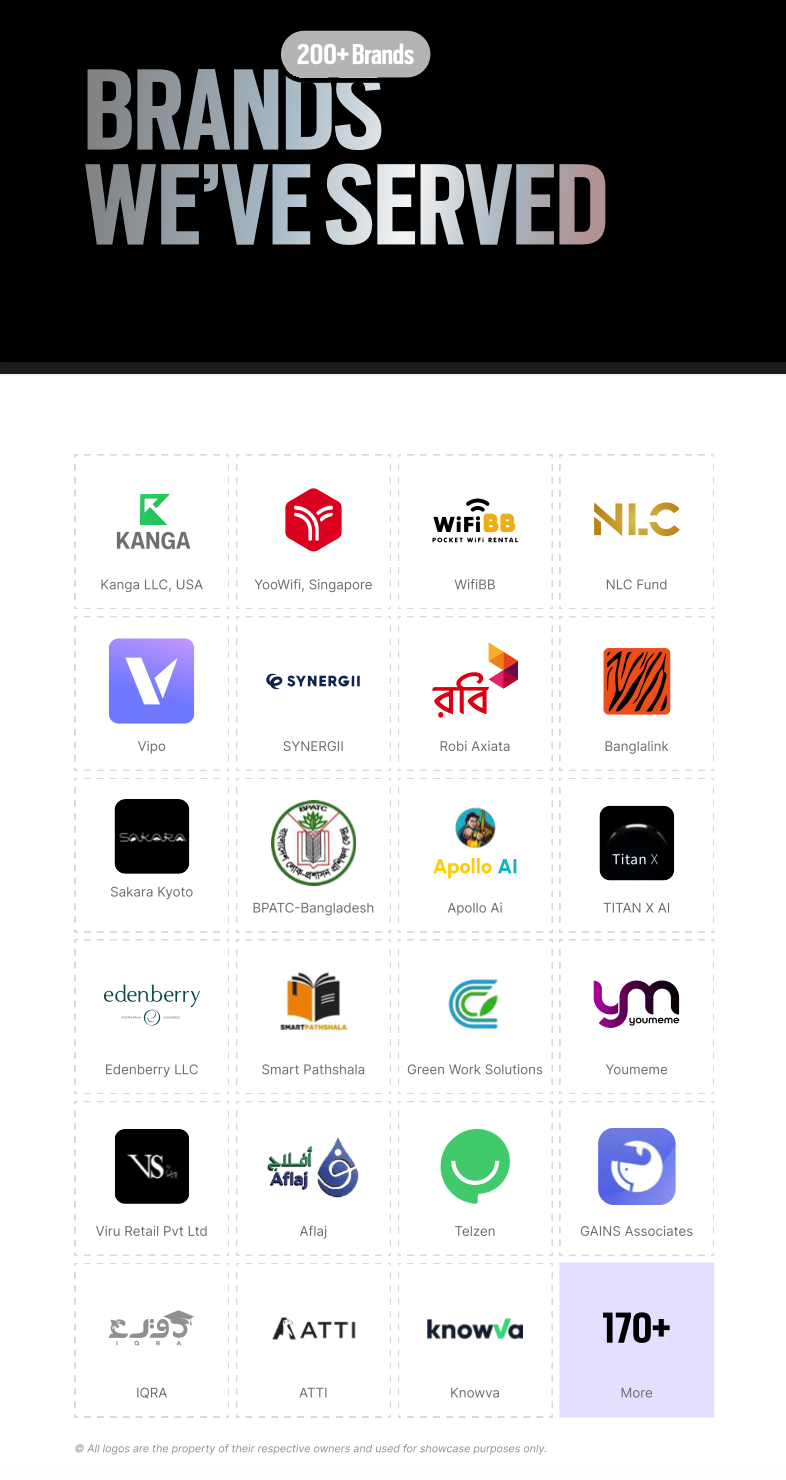
\includegraphics[width=0.6\textwidth]{Figures/served.png}
    \caption{Brands that Netro Systems Served}
\end{figure}

\newpage
\section{Company Project Portfolio}
Netro Systems has delivered a diverse portfolio of software solutions across industries. The table below summarizes several key projects, highlighting their purpose and technology stacks.

\begin{table}[h!]
\centering
\caption{Major Client Projects with Business Impact Analysis}
\label{tab:major_projects}
\begin{tabular}{p{2.2cm} p{5cm} p{3.5cm} p{3.8cm}}
\toprule
\tableheaderrow \textcolor{headertext}{\textbf{Project}} & \textcolor{headertext}{\textbf{Description}} & \textcolor{headertext}{\textbf{Industry/Country}}  & \textcolor{headertext}{\textbf{Business Outcome}} \\
\midrule
\tablealtrow \project{Smart Pathshala} & School automation platform with admin-teacher-parent modules & EdTech/Bangladesh & Reduced manual paperwork by 90\% \\
\project{Kanga} & Booking platform for home and travel services & Service Automation/USA & Increased customer retention by 6x \\
\tablealtrow \project{JazakAllah} & Islamic app with AI prayer and donation features & Lifestyle/Germany & Enhanced community engagement \\
\project{YooWifi (Telzen)} & Telecom management solution for wireless internet users & Telecom/Singapore & Improved user connectivity \\
\tablealtrow \project{NLC Fund} & Loan automation system for US-based fintech & FinTech/USA & Reduced processing time by 40\% \\
\project{DreamPath} & AI-based dream interpretation app & AI/Wellness/Global & Achieved viral adoption in beta \\
\tablealtrow \project{Trivialy} & WordPress plugin for eCommerce gamification & eCommerce/Global & Increased conversion by 40\% \\
\bottomrule
\end{tabular}
\end{table}

\newpage
\begin{figure}[h!]
\centering
\begin{subfigure}[b]{0.43\textwidth}
    \centering
    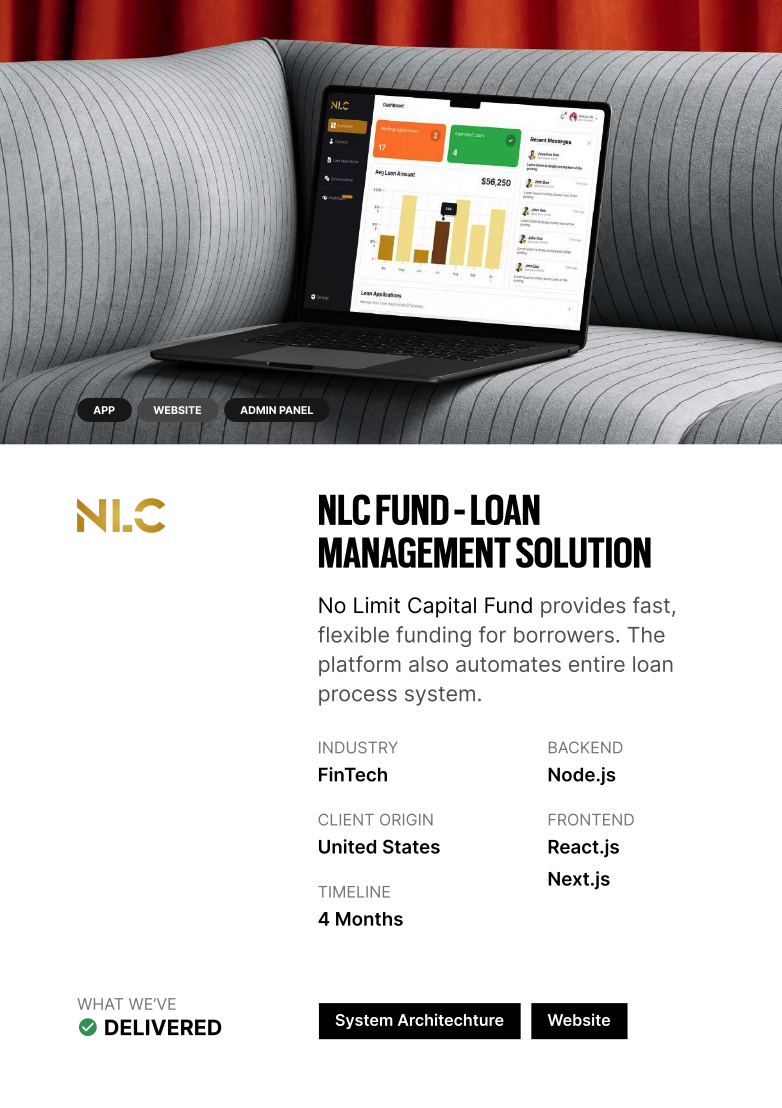
\includegraphics[width=\textwidth]{Figures/nlc.png}
    \caption{NLC Fund}
\end{subfigure}
\hfill
\begin{subfigure}[b]{0.43\textwidth}
    \centering
    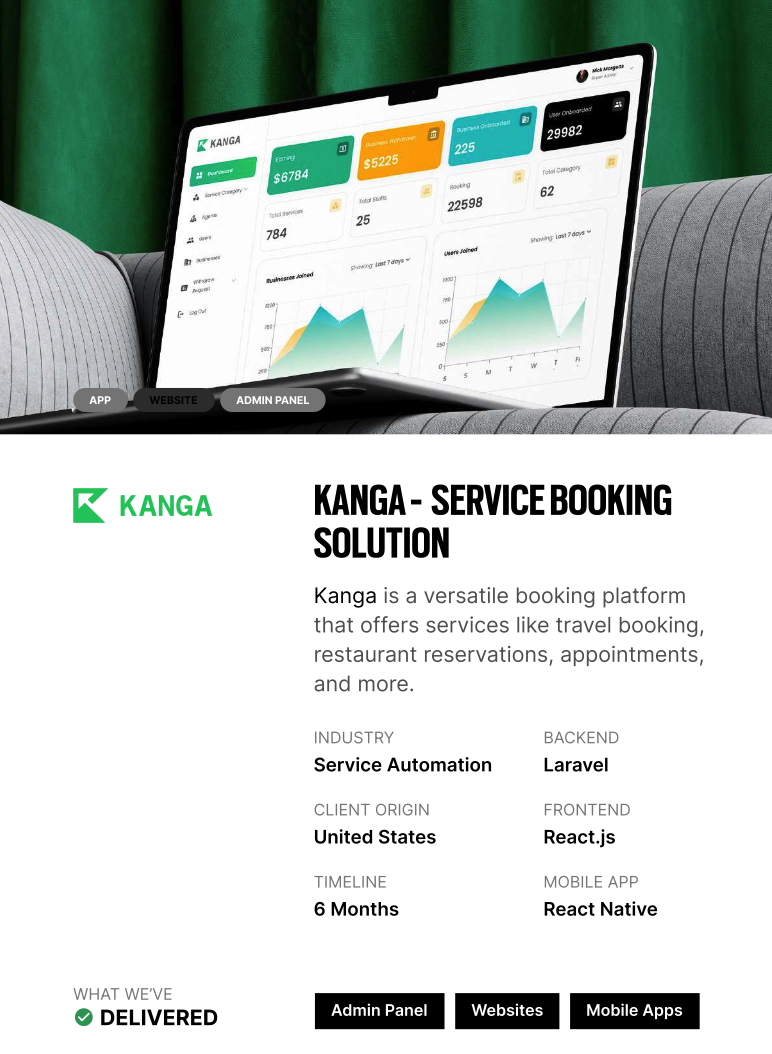
\includegraphics[width=\textwidth]{Figures/kanga.png}
    \caption{Kanga Booking}
\end{subfigure}

\vspace{0.5cm}

\begin{subfigure}[b]{0.43\textwidth}
    \centering
    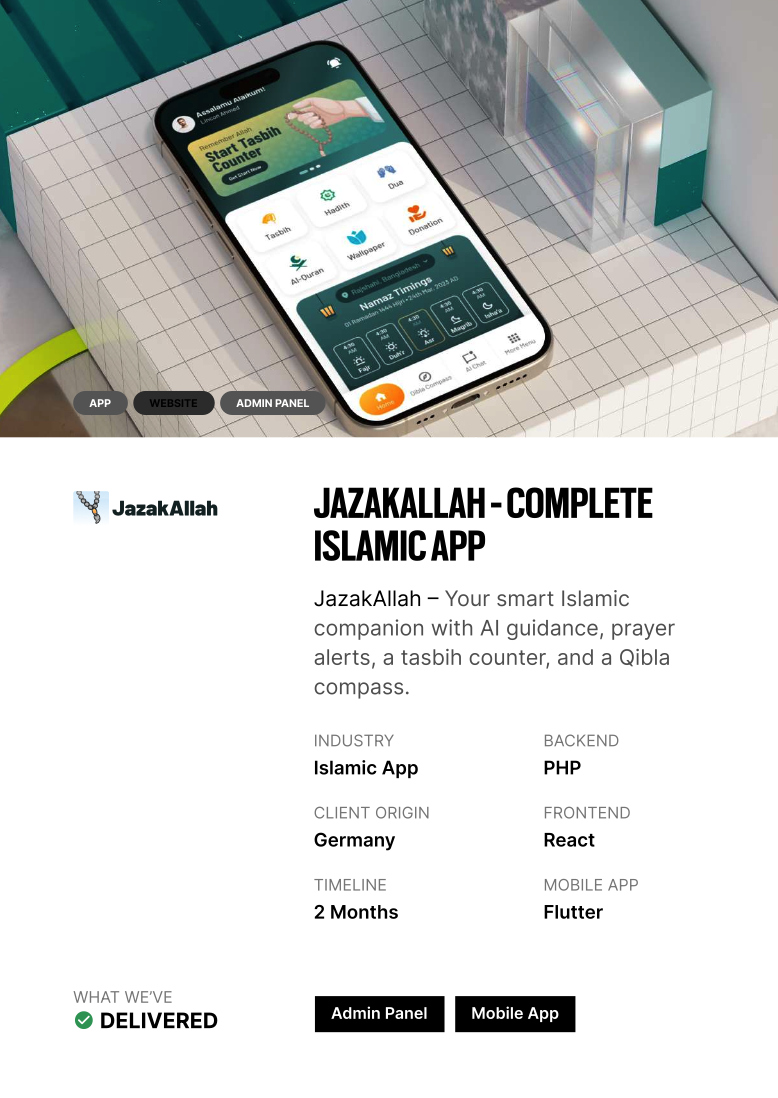
\includegraphics[width=\textwidth]{Figures/jazakallah.png}
    \caption{JazakAllah}
\end{subfigure}
\hfill
\begin{subfigure}[b]{0.43\textwidth}
    \centering
    
\includegraphics[width=\textwidth]{Figures/yoowifi.png}
    \caption{YooWifi}
\end{subfigure}

\caption{Projects Developed by Netro Systems}
\label{fig:projects_grid}
\end{figure}


\newpage
\subsection{AI and Innovation Projects}
Netro Systems has established itself as a leader in AI integration and innovative technology solutions:

\begin{table}[h!]
\centering
\caption{AI and Innovation Project Portfolio}
\label{tab:ai_projects}
\begin{tabular}{p{4cm} p{5.5cm} p{5.5cm}}
\toprule
\rowcolor{tableheader} \textcolor{headertext}{\textbf{Project}} & \textcolor{headertext}{\textbf{Purpose \& Functionality}} & \textcolor{headertext}{\textbf{AI/Innovation Features}} \\
\midrule
\tablealtrow \project{ProChat/ProAI} & AI-powered virtual assistant for business workflow automation and intelligent document processing & Natural language processing, automated workflows, intelligent document analysis \\
\project{DreamPath} & AI-driven lifestyle and travel companion with personalized recommendations and itinerary planning & Machine learning recommendations, predictive analytics, personalized content \\
\tablealtrow \project{RimOzen} & AI-based motion video generator for creative industries and automated content creation & Computer vision, video AI, automated content generation \\
\project{BizAI} & Business intelligence and analytics platform with predictive insights and automated reporting & Advanced data analytics, predictive modeling, automated business intelligence \\
\tablealtrow \project{Titan X AI} & Wearable device integration platform with health monitoring and smart notifications & AI-powered health analytics, device synchronization, predictive health insights \\
\project{Kronos AI} & Marketing automation and growth analytics with customer behavior prediction & Customer behavior analysis, automated campaign optimization, growth forecasting \\
\bottomrule
\end{tabular}
\end{table}

\begin{figure}[h!]
\centering
    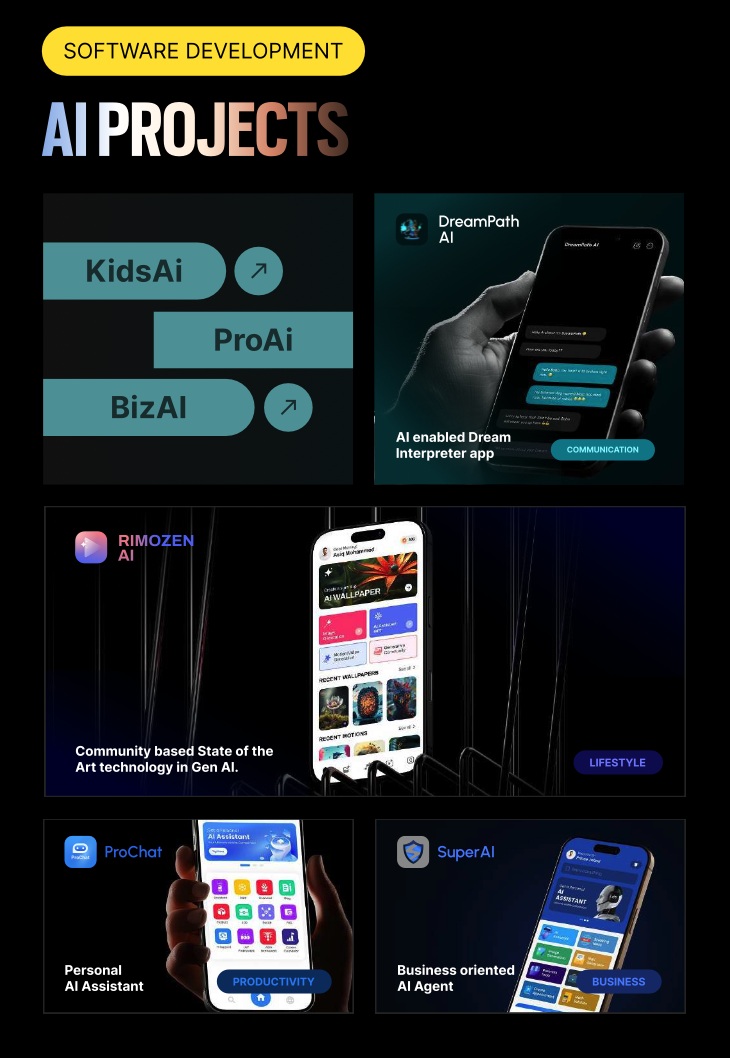
\includegraphics[width=0.26\textwidth]{Figures/ai.png}
    \caption{AI and Innovation Projects}
\end{figure}

\subsection{Client Satisfaction and Quality Metrics}
Netro Systems maintains exceptional client satisfaction rates and industry recognition:

\begin{table}[h!]
\centering
\caption{Client Satisfaction and Platform Ratings}
\label{tab:client_satisfaction}
\begin{tabular}{p{3.5cm} p{2.5cm} p{7cm}}
\toprule
\tableheaderrow \textcolor{headertext}{\textbf{Platform}} & \textcolor{headertext}{\textbf{Rating}} & \textcolor{headertext}{\textbf{Recognition Details}} \\
\midrule
\tablealtrow \impact{Clutch.co} & \textbf{5.0/5.0} & Perfect rating based on client reviews and project delivery excellence \\
\impact{GoodFirms} & \textbf{4.5/5.0} & High rating for software development and technical expertise \\
\tablealtrow \impact{Trustpilot} & \textbf{5.0/5.0} & Excellent client testimonials and service quality recognition \\
\impact{Client Retention} & \textbf{85\%+} & High repeat business rate demonstrating long-term client satisfaction \\
\tablealtrow \impact{Project Success Rate} & \textbf{98\%+} & On-time, on-budget project delivery with quality standards \\
\bottomrule
\end{tabular}
\end{table}

\section{Notable Achievements and Business Impact}
Netro Systems has established itself as a results-driven technology partner, with a proven track record of delivering transformative business outcomes for clients worldwide.

\subsection{Portfolio Statistics and Growth Metrics}
\begin{coloritemize}
    \item \skill{200+ Global Brands Served:} Successfully delivered solutions to clients across North America, Europe, Middle East, and Asia
    \item \skill{Multiple 5-Star Client Testimonials:} Consistently high client satisfaction ratings for project delivery and quality
    \item \skill{Startup Success Stories:} Helped secure \$110,000 seed funding for a startup client through strategic product development
    \item \skill{Traffic Growth Achievement:} Delivered up to 6x increase in website visitor traffic for clients after system optimization
    \item \skill{User Base Expansion:} Achieved up to 8x increase in user base for client applications post-deployment
    \item \skill{Sales Growth:} Documented exponential sales growth for international clients following system launches
\end{coloritemize}

\subsection{Industry Recognition and Awards}
\begin{coloritemize}
    \item \skill{UI/UX Innovation:} Recognized for exceptional user interface design and user experience innovation
    \item \skill{SaaS Scalability:} Acknowledged for developing highly scalable Software-as-a-Service architectures
    \item \skill{Client Success Stories:} Multiple featured case studies highlighting successful business transformations
    \item \skill{Global Partnership:} Established as a trusted technology partner for international brands
\end{coloritemize}

\begin{figure}[h!]
\centering
    
\includegraphics[width=0.5\textwidth]{Figures/awards.png}
    \caption{Awards Achieved By Netro Systems}
\end{figure}
\newpage

\section{Workplace Safety and Environmental Policy}
Netro Systems operates primarily in an office environment with standard safety measures. Offices are equipped with fire extinguishers and clearly marked emergency exits. New employees receive basic safety training, including fire drills. Given the sedentary nature of software work, ergonomic furniture (adjustable chairs, monitor stands) is provided to prevent strain injuries. Hygiene practices (sanitized desks, clean facilities) are enforced, contributing to a healthy work environment. For remote work, employees are given guidelines for safe home office setup. Environmentally, the company encourages electronic documentation to minimize paper use. Idle hardware is powered down when not needed, and e-waste is responsibly recycled. By using cloud hosting (e.g. AWS \cite{ref7}) instead of heavy local servers, Netro reduces its physical energy footprint. During my attachment, I also promoted paperless workflows in the Smart Pathshala project (e.g. digital report cards), supporting the company’s sustainability mindset.

\chapter{Project Work and Activities}

\section{Project Title and Description}
During my industrial attachment at Netro Systems, Rajshahi, I had the opportunity to learn about one of their major software products named \project{Smart Pathshala} \cite{ref2}. It is a school
management system designed to simplify academic and administrative tasks for schools,
colleges, and coaching centers in Bangladesh.
Smart Pathshala digitalizes traditional school operations such as attendance, exam
results, teacher management, accounts, student records, and communication between
teachers, guardians, and students. It includes a web portal and Android app, making it
easier for teachers and parents to access information anytime.
The main aim of this system is to reduce paperwork, save time, and increase trans-
parency between schools and parents.

\begin{figure}[h!] 
\centering 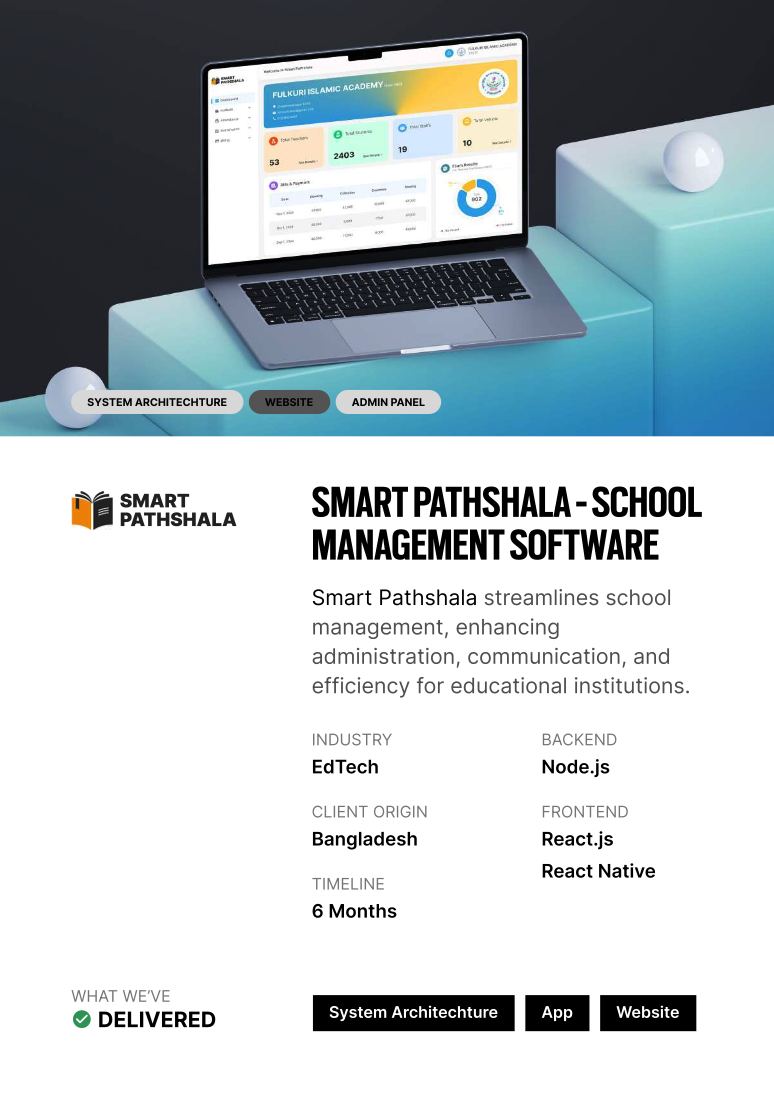
\includegraphics[width=0.35\textwidth]{Figures/smart_pathshala.png} \caption{Smart Pathshala}
\end{figure}

\section{Problem Identification \& Complexity Analysis}
Many local schools in Bangladesh rely on paper records and disconnected spreadsheets, leading to errors and inefficiency. The core problem was the lack of a centralized information system: attendance data had to be manually entered multiple times, fee records were difficult to reconcile, and communication between teachers and parents was slow. From a technical perspective, the project’s complexity included handling multiple user roles (administrators, teachers, parents, students) each with specific permissions and interfaces. The system needed real-time updates (e.g. instant notifications for absences), multilingual support (English and Bengali), and high data security (protecting student information). Ensuring scalability (for many concurrent users) and data consistency across modules added further complexity.

\section{Literature Survey and Background}
The developers studied global school management systems such as Fedena, MySchool, and OpenEduCat, but found them unsuitable for small local schools due to high cost and system complexity. They also analyzed existing educational management practices in Bangladesh—especially in rural areas—and identified key functional and contextual requirements such as:

\begin{coloritemize}
    \item Bangla-language interface to ensure inclusivity and usability among local educators and administrators.
    \item Offline access support to enable continued operation during internet outages, a common issue in remote areas.
\end{coloritemize}

Hence, \project{Smart Pathshala} was designed as a localized, user-friendly, and affordable solution tailored specifically for Bangladeshi educational institutions.


\section{Problem-Solving Approach}
The development of Smart Pathshala followed an \textbf{Agile \cite{ref8} Methodology} with iterative sprints. Our approach included:
\begin{coloritemize}
    \item \textcolor{secondaryblue}{\textbf{Requirement Analysis:}} We documented user stories (e.g., “As a teacher, I want to record daily attendance so that I can track student presence”) and defined the project scope accordingly.
    \item \textcolor{secondaryblue}{\textbf{Prototyping:}} We created wireframes and UI mockups in Figma for key modules (attendance dashboard, enrollment forms). These prototypes were reviewed by actual teachers and administrators for feedback before coding.
    \item \textcolor{secondaryblue}{\textbf{Sprint Planning:}} Work was divided into two-week sprints. Each sprint targeted a set of features – for example, one sprint developed the student registration module, another implemented the attendance management interface.
    \item \textcolor{secondaryblue}{\textbf{Iterative Development:}} Backend APIs (built with Node.js) and frontend components (React) were developed in tandem. After each sprint, we delivered a working demo to stakeholders for validation.
    \item \textcolor{secondaryblue}{\textbf{Continuous Feedback:}} Feedback from teachers and the project team was incorporated after each iteration. For example, early user tests led to UI improvements (streamlining form fields) and adjusting notification frequency.
\end{coloritemize}

\section{Experiment/Design Methodology}
The system architecture was designed using the Model-View-Controller (MVC) pattern. The backend (controller/model) runs on Node.js \cite{ref5} with Express framework and connects to a MongoDB database. The frontend (view) is built with React.js \cite{ref3} for the web portal and React Native for the mobile app, ensuring cross-platform compatibility. Key elements of our methodology included:
\begin{coloritemize}
    \item \textcolor{secondaryblue}{\textbf{Design Models:}} We created UML diagrams and database schema designs early in the process to define data entities (students, classes, attendance records) and relationships (one-to-many, etc.).
    \item \textcolor{secondaryblue}{\textbf{Version Control:}} All source code was managed with Git on GitHub. We used feature branches and pull requests; changes were peer-reviewed before merging into the main branch.
    \item \textcolor{secondaryblue}{\textbf{Testing:}} Unit tests were written using Jest for backend logic and React components. End-to-end tests using Postman(for APIs) and React Testing Library (for UI) helped catch integration issues early. 
    \item \textcolor{secondaryblue}{\textbf{Hosting \& Deployment:}} AWS \cite{ref7} Cloud for stability and scalability; Docker for containerization.
\end{coloritemize}

\newpage
\section{Validation of Findings}
\label{sec:validation}
\project{Smart Pathshala} was tested in several schools located in Rajshahi and Dhaka to evaluate its usability, performance, and overall effectiveness. The key findings from the pilot implementation are summarized below:

\begin{coloritemize}
    \item \textcolor{secondaryblue}{\textbf{Reduced manual work:}} Attendance and exam results could be entered within minutes, significantly reducing administrative workload for teachers.
    \item \textcolor{secondaryblue}{\textbf{Higher accuracy:}} Automated report generation minimized human errors and ensured consistent data recording.
    \item \textcolor{secondaryblue}{\textbf{Better communication:}} Parents could instantly view their children’s attendance, fee status, and exam results through the mobile application, improving engagement.
    \item \textcolor{secondaryblue}{\textbf{Positive user feedback:}} Teachers found the interface intuitive and user-friendly, while parents appreciated real-time updates and transparency.
    \item \textcolor{secondaryblue}{\textbf{Performance:}} The system efficiently handled thousands of student records without noticeable lag, validating its scalability and robustness.
\end{coloritemize}

Overall, \project{Smart Pathshala} proved to be an effective and reliable school management solution tailored to the context of Bangladeshi educational institutions.


\chapter{Tools and Techniques}
\section{Technology Stack and Engineering Tools}
During my industrial attachment at Netro Systems, I gained extensive hands-on experience with a comprehensive suite of modern development tools, frameworks, and technologies that represent current industry standards. This diverse technology stack enabled me to contribute effectively to complex, enterprise-grade software projects while developing professional competencies in full-stack development.

\subsection{Programming Languages and Core Technologies}
\begin{coloritemize}
    \item \tool{JavaScript (ES6+):} Advanced modern JavaScript for both client-side and server-side development
    \item \tool{Node.js \cite{ref5}:} Runtime environment for scalable server-side applications and API development
    \item \tool{TypeScript:} Strongly-typed JavaScript superset for enterprise-grade application development
    \item \tool{PHP:} Server-side scripting for legacy system integration and WordPress-based solutions
    \item \tool{Python:} Data processing, AI/ML integration, and automation scripting
    \item \tool{HTML5/CSS3:} Modern web standards with responsive design principles
    \item \tool{SQL:} Database query language for relational database management
\end{coloritemize}

\newpage
\subsection{Frontend Development Frameworks and Libraries}
\begin{coloritemize}
    \item \tool{React.js \cite{ref3}:} Component-based library for building dynamic, interactive user interfaces
    \item \tool{Next.js:} React framework for server-side rendering and static site generation
    \item \tool{Vue.js:} Progressive framework for building user interfaces with component-based architecture
    \item \tool{Angular:} TypeScript-based platform for building mobile and desktop web applications
    \item \tool{Tailwind CSS:} Utility-first CSS framework for rapid UI development
    \item \tool{Bootstrap:} Responsive design framework for consistent UI components
    \item \tool{Material-UI:} React components implementing Google's Material Design
\end{coloritemize}

\subsection{Backend Technologies and Server Frameworks}
\begin{coloritemize}
    \item \tool{Express.js:} Minimal and flexible Node.js web application framework
    \item \tool{Laravel:} PHP framework for robust web application development
    \item \tool{Django:} Python web framework following the model-template-views architectural pattern
    \item \tool{FastAPI:} Modern, fast Python web framework for building APIs
\end{coloritemize}

\subsection{Mobile Development Technologies}
\begin{coloritemize}
    \item \tool{React Native:} Cross-platform mobile development using React principles
    \item \tool{Flutter \cite{ref4}:} Google's UI toolkit for building natively compiled applications
    \item \tool{Expo:} Platform for universal React applications with streamlined development workflow
\end{coloritemize}

\subsection{Database Management Systems}
\begin{coloritemize}
    \item \tool{MongoDB:} NoSQL document database providing flexibility and scalability
    \item \tool{PostgreSQL \cite{ref6}:} Advanced open-source relational database with extensive feature set
    \item \tool{MySQL:} Widely-used relational database management system
    \item \tool{Firebase:} Google's mobile and web application development platform
\end{coloritemize}

\subsection{Development Tools and Environment}
\begin{coloritemize}
    \item \tool{Visual Studio Code:} Primary IDE with extensive extension ecosystem
    \item \tool{WebStorm:} JetBrains IDE for JavaScript and web development
    \item \tool{Git:} Distributed version control system for source code management
    \item \tool{GitHub/GitLab:} Cloud-based Git repositories with collaboration features
    \item \tool{Docker:} Containerization platform for consistent development environments
    \item \tool{Postman:} API development and testing platform
\end{coloritemize}

\subsection{Testing and Quality Assurance Tools}
\begin{coloritemize}
    \item \tool{Jest:} JavaScript testing framework with zero configuration
    \item \tool{Cypress:} End-to-end testing framework for web applications
    \item \tool{Selenium:} Web browser automation for functional testing
    \item \tool{React Testing Library:} Testing utilities for React components
    \item \tool{Prettier:} Code formatter for maintaining consistent code style
\end{coloritemize}

\subsection{Design and Prototyping Tools}
\begin{coloritemize}
    \item \tool{Figma:} Collaborative interface design and prototyping platform
    \item \tool{Adobe XD:} Vector-based user experience design tool
    \item \tool{Adobe Creative Suite:} Professional design software including Photoshop and Illustrator
\end{coloritemize}

\subsection{Project Management and Collaboration}
\begin{coloritemize}
    \item \tool{Jira:} Agile \cite{ref8} project management and issue tracking platform
    \item \tool{Trello:} Visual project management tool using Kanban boards
    \item \tool{Zoom:} Team communication and collaboration platform
    \item \tool{Microsoft Teams:} Unified communication and collaboration platform
    \item \tool{Notion:} All-in-one workspace for notes, documentation, and project management
\end{coloritemize}

\subsection{Cloud Services and DevOps Tools}
\begin{coloritemize}
    \item \tech{Amazon Web Services (AWS) \cite{ref7}:} Comprehensive cloud computing platform
    \item \tech{Google Cloud Platform:} Suite of cloud computing services
    \item \tech{Microsoft Azure:} Cloud computing service for building and managing applications
    \item \tech{Netlify:} Platform for deploying and hosting static websites and web applications
    \item \tech{Vercel:} Cloud platform for static sites and serverless functions
    \item \tool{Jenkins:} Open-source automation server for CI/CD pipelines
    \item \tool{GitHub Actions:} Native CI/CD platform integrated with GitHub repositories
\end{coloritemize}


\begin{table}[h!]
\centering
\caption{Netro Systems Technology Stack Overview}
\label{tab:tech_ecosystem}
\begin{tabular}{@{}p{7cm}p{8cm}@{}}
\toprule
\tableheaderrow \textcolor{headertext} {\textbf{Technology Domain}} & \textcolor{headertext} {\textbf{Key Technologies}} \\
\midrule
\impact{Frontend Development} & \tech{React.js, Vue.js, Angular, TypeScript, HTML5, CSS3} \\
\tablealtrow \impact{Backend Development} & \tech{Node.js, Express.js, PHP Laravel, Python Django, RESTful APIs} \\
\impact{Mobile Development} & \tech{React Native, Flutter, Swift (iOS), Kotlin (Android)} \\
\tablealtrow \impact{Database Management} & \tech{MongoDB, PostgreSQL, MySQL, Firebase Realtime Database} \\
\impact{Cloud \& DevOps} & \tech{AWS \cite{ref7} Services, Docker, GitHub Actions} \\
\tablealtrow \impact{Design \& Prototyping} & \tech{Figma, Adobe XD, Adobe Illustrator} \\
\bottomrule
\end{tabular}
\end{table}


\section{Application in Solving Complex Problems}
These tools were instrumental in solving engineering challenges. For example, React’s component-based structure made it easier to manage complex UIs (e.g. reusing form components for student and teacher dashboards). MongoDB’s query flexibility allowed generating reports (like monthly attendance) directly via its aggregation framework. Git branching enabled team members to work on different features (attendance vs. grading) concurrently without conflict. CI pipelines (Jenkins/GitHub Actions) automatically ran tests on every commit, quickly alerting us to integration issues before they could affect other parts of the project.

\newpage
\section{Limitations and Constraints}
Every tool had some constraints, such as-
\begin{coloritemize}
    \item \textbf{\tool{Scalability:}} While MongoDB scales well, it required careful indexing as the number of records (students, attendance entries) grew. We experienced slower queries initially until indexes were optimized.
    \item \textbf{\tool{Learning Curve:}} As an intern, learning both Node.js and React from scratch was challenging, delaying initial productivity. This was mitigated by team mentorship and online resources, which rapidly improved my proficiency.
    \item \textbf{\tool{Third-party Integrations:}} Integrating external APIs (e.g. SMS gateway for notifications) introduced dependency management issues (version conflicts). We handled this by using npm and thorough testing to catch conflicts early.
    \item \textbf{\tool{Testing Tools:}} Setting up the testing infrastructure (Jest, Selenium) required upfront configuration. Although time-consuming at first, this investment paid off by catching defects early in development.
\end{coloritemize}

\section{Simulation and Testing Tools}
To verify system performance and correctness, we used:
\begin{coloritemize}
    \item \textbf{\tool{Postman}:} For manual API testing. I simulated requests from different user roles (teacher, admin, parent) to verify correct responses and error handling.
    \item \textbf{\tool{Jest \&}} \textbf{\tool{Enzyme}:} For automated unit testing of backend logic and React components. These tests were configured to run on every pull request.
    \item \textbf{\tool{Docker}:} Used to create containers replicating the production environment. This ensured consistency between my local setup and the deployment server, minimizing “it works on my machine” issues.
    \item \textbf{\tool{Apache JMeter}:} Performed basic load testing on our APIs. The system handled anticipated concurrent user loads smoothly, confirming our scaling strategy for a school setting.
\end{coloritemize}

\chapter{Societal, Health, Safety, Legal \& Cultural Considerations}
\section{Workplace, Health and Safety Measures}
During my attachment at Netro Systems, Rajshahi, I observed that the company main-
tains a professional and safe working environment. The office followed standard health
and safety practices to ensure employee well-being.\\
The workspace was clean, well-lit, and air-conditioned, with comfortable seating suit-
able for long hours of computer work. Developers often spend most of their time sitting
in front of screens, so ergonomic chairs and adjustable desks were provided to prevent
back and neck pain. The team encouraged short breaks to reduce eye strain and improve
concentration.\\
Senior-junior bonding has been found out quite a good unlike the others in Bangladesh.
There is no separate working desk for senior and junior worker of a single team. Rather,
all of them sit together and share their valuable knowledge while working. Boys and girls
members have given separate workspace so that they can work comfortably.\\
Safety measures included accessible fire extinguishers, organized electrical wiring to
avoid hazards, clearly marked emergency exits, and visible safety instructions. Hand
sanitizers were available at every corner, especially important after the COVID-19 period.
Digital safety was also emphasized. Each workstation had antivirus software, and
internet usage was monitored to prevent cybersecurity risks. The internal Wi-Fi network
was protected with password authentication to avoid unauthorized access to company
files.

\subsection{Physical Work Environment}
\begin{coloritemize}
    \item \feature{Ergonomic Infrastructure:} Modern office spaces equipped with adjustable desks, ergonomic chairs, and proper lighting to prevent repetitive strain injuries
    \item \feature{Safety Protocols:} Comprehensive safety measures including clearly marked emergency exits, fire safety equipment, and regular safety drills
    \item \feature{Health and Hygiene:} Sanitized workstations, clean facilities, and well-maintained kitchen areas promoting overall health and well-being
    \item \feature{Technology Resources:} High-performance workstations, multiple monitor setups, and reliable internet connectivity for optimal productivity
\end{coloritemize}

\subsection{Work Culture and Environment}
\begin{table}[h!]
\centering
\caption{Workplace Culture and Employee Benefits}
\label{tab:workplace_culture}
\begin{tabular}{p{5.5cm} p{8.5cm}}
\toprule
\tableheaderrow \textcolor{headertext}{\textbf{Aspect}} & \textcolor{headertext}{\textbf{Description}} \\
\midrule
\tablealtrow \impact{Work Model} & Flexible hybrid work environment with options for remote work and flexible hours \\
\skill{Professional Development} & Continuous learning opportunities, internal training sessions, and access to online courses \\
\tablealtrow \tool{Collaboration Tools} & Modern communication platforms including Slack, Zoom, and collaborative project management tools \\
\feature{Team Building} & Regular team-building activities, lunch-and-learn sessions, and knowledge sharing initiatives \\
\tablealtrow \tech{Innovation Culture} & Encouragement of creative problem-solving, experimentation with new technologies, and innovation projects \\
\impact{Diversity \& Inclusion} & Inclusive hiring practices, cultural sensitivity training, and respect for diverse backgrounds \\
\bottomrule
\end{tabular}
\end{table}

\subsection{Remote Work Support}
\begin{coloritemize}
    \item \skill{Home Office Guidelines:} Comprehensive guidelines for setting up ergonomic and productive home workstations
    \item \skill{Digital Collaboration:} Advanced tools and platforms for seamless remote collaboration and communication
    \item \skill{Work-Life Balance:} Flexible scheduling policies that respect personal time and promote healthy work-life integration
    \item \skill{Technical Support:} IT support and necessary equipment provision for remote workers
\end{coloritemize}

\newpage
\begin{figure}[h!] 
\centering 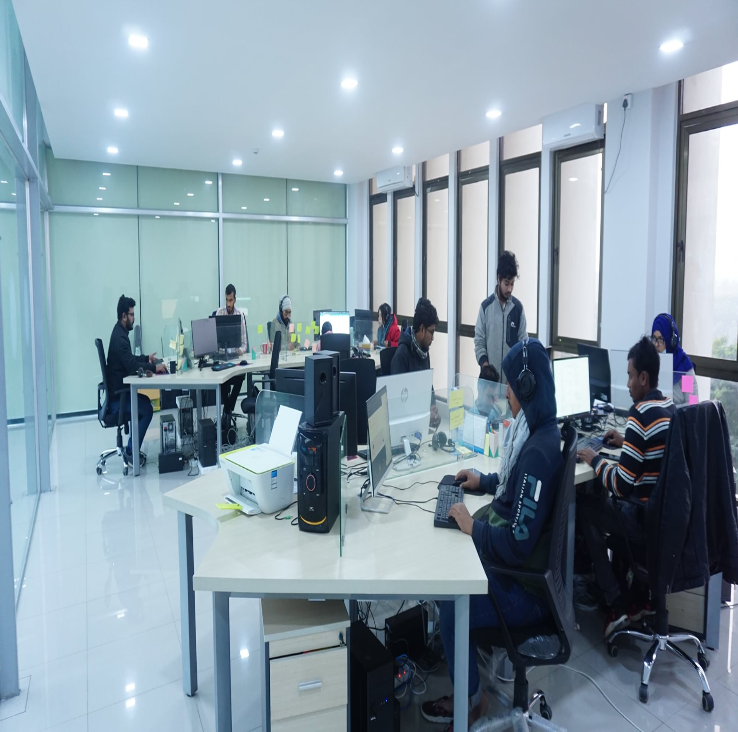
\includegraphics[width=0.5\textwidth]{Figures/workplace.png} \caption{Workplace of Netro Systems}
\end{figure}

\section{Legal Compliance in Engineering Activities}
\company{Netro Systems Limited} strictly follows all legal and regulatory guidelines relevant to software development and data management in Bangladesh. Before initiating any project, the company executes a formal legal deed with the client, clearly defining deliverables, timelines, intellectual property rights, and update or maintenance responsibilities. Confidentiality is a core value—project information is never shared with external parties without authorization.

For \project{Smart Pathshala}, which involves sensitive student data, the company implemented several legal and ethical compliance measures to ensure data protection and integrity:

\begin{coloritemize}
    \item \textcolor{skillcolor}{\textbf{Licensed and open-source tools:}} All software tools and libraries used were either properly licensed or open-source with permissible usage rights.
    \item \textcolor{skillcolor}{\textbf{Data privacy and security:}} Sensitive data, including student profiles and fee records, were encrypted using secure algorithms to prevent unauthorized access.
    \item \textcolor{skillcolor}{\textbf{Confidentiality agreements:}} All clients and collaborators signed Non-Disclosure Agreements (NDAs) to maintain confidentiality of proprietary information.
    \item \textcolor{skillcolor}{\textbf{Controlled data access:}} Internal data access policies strictly limited who could view or modify production databases, ensuring accountability.
\end{coloritemize}

These practices demonstrate that professional software engineering \cite{ref11} extends beyond technical development—it encompasses ethical, legal, and regulatory responsibilities to safeguard user data and intellectual property.

\section{Societal, Cultural Awareness in Solution Design}
Netro Systems' global client base requires deep understanding of diverse cultural contexts and societal needs. During my attachment, I observed how the company integrates cultural sensitivity into solution design:

\subsection{Cross-Cultural Design Considerations}
\begin{coloritemize}
    \item \skill{Multilingual Support:} Smart Pathshala was designed with Bengali and English language support, recognizing the linguistic diversity in Bangladesh's educational sector
    \item \skill{Local Educational Standards:} The system accommodated Bangladesh's specific academic calendar, grading systems, and regulatory requirements
    \item \skill{Cultural Accessibility:} User interface design considered local preferences for color schemes, layout patterns, and navigation structures
    \item \skill{Religious Considerations:} The JazakAllah project demonstrated sensitivity to Islamic cultural practices with prayer time calculations and Qibla direction features
\end{coloritemize}

\subsection{Digital Divide and Accessibility}
\begin{coloritemize}
    \item \skill{Low-Bandwidth Optimization:} Applications are optimized for slower internet connections common in developing markets
    \item \skill{Mobile-First Design:} Recognizing higher mobile device penetration compared to desktop computers in many target markets
    \item \skill{Offline Functionality:} Critical features designed to work without constant internet connectivity
    \item \skill{Economic Accessibility:} Solutions priced appropriately for local economic conditions and purchasing power
\end{coloritemize}
Smart Pathshala’s design was influenced by societal and cultural factors. For example, the interface supports both English and Bengali languages to accommodate local users. Recognizing diverse levels of digital literacy, the UI was kept clean and intuitive (large buttons, clear icons). We aligned the school calendar with local norms (incorporating regional holidays). During development, I realized that understanding the user’s cultural context is key: for instance, notifications and reports avoided culturally sensitive content, and color choices were made with local preferences in mind. This cultural awareness improved user acceptance of the solution.

\section{Environmental Sustainability Considerations}
Netro Systems is conscious of environmental impact in its operations. The company uses cloud hosting (AWS \cite{ref7}) rather than on-site servers, reducing hardware energy usage. Idle servers and devices are powered down when not needed. E-waste (old laptops, hard drives) is recycled through approved channels. Internally, digital documentation is encouraged over printing. While working on Smart Pathshala, we also promoted paperless practices in schools (e.g. electronic report cards and notices), indirectly contributing to sustainability by saving paper. These practices reflect an understanding of the environmental footprint of software systems.

\section{Case Examples from the Attachment Site}
During my attachment at \company{Netro Systems Limited}, several practical examples illustrated how legal, ethical, health, cultural, and environmental considerations were integrated into daily engineering practice. The following cases highlight key insights:

\begin{coloritemize}
    \item \textcolor{secondaryblue}{\textbf{Case 1 – Health and Ergonomics:}} Developers were encouraged to take regular breaks every hour to reduce fatigue and improve focus, resulting in higher productivity and well-being.
    
    \item \textcolor{secondaryblue}{\textbf{Case 2 – Legal Awareness:}} A free online resource library was removed due to licensing restrictions, emphasizing the importance of respecting intellectual property rights and software ownership.
    
    \item \textcolor{secondaryblue}{\textbf{Case 3 – Cultural Inclusion in Design:}} Bangla fonts were updated to Unicode-supported versions, ensuring accurate text rendering and accessibility on older and diverse devices.
    
    \item \textcolor{secondaryblue}{\textbf{Case 4 – Environmental Impact of Digitalization:}} Transitioning from paper-based attendance sheets to digital records helped save approximately 1,000 paper sheets per school per month—scaling this across institutions results in significant environmental benefits.
\end{coloritemize}

These case examples reinforce how professional engineering practice must integrate legal, cultural, environmental, and ergonomic awareness to achieve sustainable and ethically sound technological development.


\chapter{Professional Ethics \& Responsibilities}
\section{Ethical Issues Faced During the Attachment}
During my attachment at Netro Systems, I realized that ethics plays a major role in pro-
fessional software development. In the Smart Pathshala project, several ethical concerns
needed attention. The system stores sensitive student and school information, including
attendance, academic records, and financial details. Therefore, maintaining data privacy
and confidentiality was a top priority.\\

Developers were instructed not to access or view real user data unless necessary for
debugging. Every action involving production data required prior permission from the
project manager. Ethical behavior also meant not copying code or using third-party
software without proper licenses. A regular meeting in a week is conducted to educate
the team members about all of the concerning matters and it shows how Netro System
takes importance regarding this issue.\\

I also learned about ethical coding practices — writing clean, readable code, avoiding
shortcuts that could cause future problems, and documenting properly. All these steps
reflected professional integrity and responsibility

\section{Professional Codes of Ethics}
\company{Netro Systems Limited} adhered to both organizational and engineering ethics, consistent with the professional codes promoted by international engineering bodies such as the IEEE \cite{ref9} and the British Computer Society (BCS) \cite{ref10}. These ethical principles served as a foundation for professional behavior and guided decision-making throughout project development.

\newpage
\begin{coloritemize}
    \item \textcolor{secondaryblue}{\textbf{Honesty:}} Team members maintained transparency about project progress, challenges, and outcomes, ensuring truthful communication with clients and supervisors.
    \item \textcolor{secondaryblue}{\textbf{Accountability:}} Developers accepted responsibility for mistakes or system issues, working collaboratively to identify root causes and implement corrective actions.
    \item \textcolor{secondaryblue}{\textbf{Fairness:}} Equal opportunities were provided to all team members, with recognition based on merit and contribution rather than hierarchy or personal bias.
    \item \textcolor{secondaryblue}{\textbf{Respect:}} Clients, users, and colleagues were treated with courtesy, and their feedback was valued in decision-making processes.
    \item \textcolor{secondaryblue}{\textbf{Integrity:}} Software was developed and delivered with authenticity, avoiding false claims, plagiarism, or unethical manipulation of deliverables.
\end{coloritemize}

Every intern and employee at \company{Netro Systems Limited} was expected to uphold these standards. During meetings, I observed that team members consistently avoided exaggeration and reported the actual status of work, even when delays occurred. This culture of honesty and transparency built a strong sense of trust and professionalism within the team.


\section{Intellectual Property and Confidentiality}
Netro Systems maintains strict confidentiality of client information. All code and documentation were stored in secured repositories with controlled access. I treated all project materials (code, designs, data) as proprietary. Intellectual property issues were managed by using properly licensed libraries (avoiding unlicensed code) and by clear contracts ensuring any custom work done by interns belongs to the company. This clear IP framework meant I focused on innovation without concerns about ownership.

\section{Ethical Decision-Making Examples}
An example of ethical decision-making occurred when I discovered an unlicensed third-party code snippet in one of our dependencies. I immediately reported it to my supervisor. Together, we replaced it with a fully open-source alternative and documented the change, avoiding any infringement. In another instance, deciding how much personal data to collect was an ethical consideration: I limited data fields to only what was essential, respecting privacy principles. These decisions show applying ethical reasoning in engineering tasks.

\chapter{Skills Gained \& Lifelong Learning}

\section{Technical Skills Gained}
During my industrial attachment at \company{Netro Systems Limited}, I gained a wide range of practical technical knowledge that has significantly enhanced my understanding of real-world software engineering \cite{ref11} practices. Observing the development teams across several projects helped me comprehend the professional workflow and coordination involved in delivering high-quality software solutions. The main technical skills I learned include:

\begin{coloritemize}
    \item \textcolor{secondaryblue}{\textbf{Frontend Development:}} I learned how the company used React.js to build interactive, responsive, and high-performance user interfaces. I practiced tasks such as modifying small components and understanding how APIs connect the frontend to the backend systems.
    
    \item \textcolor{secondaryblue}{\textbf{Mobile Application Development:}} Through Flutter \cite{ref4}, I observed how a single codebase could serve both Android and iOS platforms. I understood how widgets, layouts, and API calls were structured to deliver consistent mobile experiences.
    
    \item \textcolor{secondaryblue}{\textbf{Backend Concepts:}} I studied how Node.js and Express.js handled API requests, user authentication, and server responses, ensuring secure and efficient data flow between client and server components.
    
    \item \textcolor{secondaryblue}{\textbf{Database Management:}} I gained exposure to PostgreSQL \cite{ref6}, the relational database used in \project{Smart Pathshala}, learning about table creation, foreign key relationships, and maintaining data integrity.
    
    \item \textcolor{secondaryblue}{\textbf{Cloud Hosting:}} I observed how the team utilized Amazon Web Services (AWS) \cite{ref7} for secure hosting and seamless deployment of project updates without downtime.
    
    \item \textcolor{secondaryblue}{\textbf{Testing and Debugging:}} I learned to test API endpoints using Postman and assisted in reporting bugs to developers. From unit to integration testing, I experienced the full testing process and its importance in maintaining software reliability.
\end{coloritemize}

\section{Soft Skills Developed}
Apart from technical proficiency, I also developed several essential soft skills during the attachment, which are vital for professional success in collaborative environments:

\begin{coloritemize}
    \item \textcolor{secondaryblue}{\textbf{Communication Skills:}} I learned to articulate technical ideas clearly during meetings and ask questions politely when clarification was needed.
    
    \item \textcolor{secondaryblue}{\textbf{Teamwork:}} I realized the significance of collaboration and mutual support. Since every team member’s progress affected the others, regular updates and cooperation were crucial for success.
    
    \item \textcolor{secondaryblue}{\textbf{Time Management:}} I learned to balance multiple responsibilities—documentation, observation, and testing—within limited timeframes.
    
    \item \textcolor{secondaryblue}{\textbf{Problem-Solving:}} Observing developers diagnose and fix complex issues taught me logical reasoning and the importance of analyzing the root cause before proposing solutions.
    
    \item \textcolor{secondaryblue}{\textbf{Presentation Skills:}} On the final day of the attachment, I presented my learning outcomes. Preparing slides and delivering the presentation improved my confidence and public speaking ability, helping me overcome nervousness.
\end{coloritemize}

\section{Adaptation to New Technologies}
Initially, I was unfamiliar with tools such as \textbf{Docker}, \textbf{Git}, and \textbf{PostgreSQL}. However, through continuous observation and guided practice, I quickly adapted to their usage. I also learned about version control with \textbf{GitHub}—how developers perform commits, push and pull operations, resolve merge conflicts, and conduct code reviews. These experiences strengthened my adaptability and technical agility, preparing me for diverse software environments.

\section{Lifelong Learning Reflection}
This industrial attachment reinforced my understanding that technology evolves rapidly. Frameworks, tools, and languages that dominate today may become obsolete within a few years. To remain competent, I must adopt a mindset of continuous learning. I have developed the habit of reading about new technologies, exploring open-source projects, and following software engineering trends through reputable industry sources. This commitment to lifelong learning will ensure I continue to grow as a capable and future-ready software engineer.


\chapter{Challenges \& Solutions}
\section{Technical Challenges}
During my industrial attachment, I encountered several challenges that tested my understanding of professional software development practices. Some of the main technical challenges and their respective solutions are described below:

\begin{coloritemize}
    \item \textcolor{secondaryblue}{\textbf{Understanding Large Codebases:}} In university projects, I typically worked on smaller, self-contained codebases. However, industry-level projects such as Smart Pathshala involved hundreds of interconnected files and modules. Initially, it was difficult to comprehend how various components interacted within the overall system architecture.\\
    
    \textbf{\skill{Solution:}} My supervisor advised me to analyze small sections of code daily and trace the data flow between the frontend and backend components, which gradually improved my understanding.
    
    \item \textcolor{secondaryblue}{\textbf{Database Errors:}} While testing data entries, I encountered issues such as duplicate records and missing fields.\\
    
    \textbf{\skill{Solution:}} I learned about database normalization principles and implemented constraints in PostgreSQL to prevent redundant or inconsistent data entries.
    
    \item \textcolor{secondaryblue}{\textbf{API Integration:}} Understanding how APIs connected the web application with the mobile application was initially challenging.\\ 
    
    \textbf{\skill{Solution:}} I used Postman to test different API endpoints and observed how responses varied with different types of requests, helping me grasp request–response mechanisms effectively.
    
    \item \textcolor{secondaryblue}{\textbf{Version Control Conflicts:}} Occasionally, developers faced Git merge conflicts when multiple people edited the same file concurrently.\\
    
    \textbf{\skill{Solution:}} I studied how Git branching strategies work and learned that maintaining clear commit messages and proper commenting beside code greatly improves collaboration and conflict resolution.
\end{coloritemize}

These challenges provided hands-on exposure to real-world software engineering problems and taught me the importance of systematic learning, collaboration, and persistence in resolving technical issues.


\section{Administrative and Organizational Issues}
Coordination was a challenge because some team members (including me) worked remotely. To address this, we scheduled overlapping hours for team meetings and relied on Zoom for daily stand-ups and quick syncs. Additionally, a late requirement change (adding a new report field) threatened our sprint plan. The team quickly held a re-planning session using Jira to update tasks and priorities, ensuring everyone understood the new goals.

\section{Lessons Learned}
These challenges taught me valuable lessons: clear and frequent communication is crucial in a distributed team, and flexibility is needed when project scope changes. The debugging experience reinforced the importance of systematic problem-solving and documentation. Overall, facing these challenges improved my resilience and ability to collaborate under pressure.

\chapter{Contribution to the Organization}

\section{Tasks Performed}
Although I was an intern, I actively contributed to the \project{Smart Pathshala} project through multiple hands-on and supportive tasks that helped the team in testing, documentation, and user feedback analysis.

\begin{coloritemize}
    \item \textcolor{secondaryblue}{\textbf{Testing Modules:}} Assisted in testing different project components, especially the attendance and exam result sections.
    \item \textcolor{secondaryblue}{\textbf{Reporting UI Issues:}} Reported small user interface and data display inconsistencies to the development team for correction.
    \item \textcolor{secondaryblue}{\textbf{Data Preparation:}} Helped prepare sample datasets such as student records for internal testing and client demonstrations.
    \item \textcolor{secondaryblue}{\textbf{Documentation Updates:}} Updated sections of the technical documentation after new features were introduced or modified.
    \item \textcolor{secondaryblue}{\textbf{Client Feedback Observation:}} Observed client feedback sessions and assisted in noting down improvement suggestions for subsequent project iterations.
\end{coloritemize}

\section{Suggestions for Improvement}
Based on my observations during the internship and feedback from end users, I proposed several improvements to enhance the user experience and functionality of \project{Smart Pathshala}.

\begin{coloritemize}
    \item \textcolor{secondaryblue}{\textbf{Interactive Dashboard Tutorial:}} Include a simple dashboard walkthrough or tutorial for first-time users to help them navigate easily.
    \newpage
    \item \textcolor{secondaryblue}{\textbf{Offline Attendance Entry:}} Introduce an offline mode for schools with unreliable internet connectivity to record attendance locally and sync when online.
    \item \textcolor{secondaryblue}{\textbf{Improved Bangla Font Support:}} Optimize Bangla font rendering on older Android devices to ensure proper display and usability.
    \item \textcolor{secondaryblue}{\textbf{AI Chatbot Integration:}} Incorporate an AI-powered chatbot in the app or website to assist users with common queries and technical support.
\end{coloritemize}

\section{Feedback from Supervisor}
My supervisor expressed satisfaction with my enthusiasm and commitment to learning. He encouraged me to continue strengthening my coding and backend development skills, particularly focusing on cloud-based systems and API design. Additionally, he advised exploring AI-integrated technologies such as Agentic AI, recognizing the growing industry trend toward intelligent automation. I was also appreciated for maintaining detailed testing documentation, effective communication, and teamwork throughout the internship.


\chapter{Conclusion \& Recommendations}
\section{Summary of the Attachment}
In conclusion, my industrial attachment at \company{Netro Systems Limited} was a rewarding experience that bridged academic studies with industry practice. I engaged in real project development and learned new tools and methodologies in the process. I contributed tangible features to the \project{Smart Pathshala} project which enhanced my problem-solving skills, and gained insight into professional software engineering \cite{ref11} workflows. The objectives set at the start were met: I learned modern technologies (React, Node.js), understood the software development lifecycle, and experienced a collaborative work environment.

\section{Recommendations}
Based on this valuable industrial attachment, I offer the following recommendations:

\subsection{For Netro Systems Limited}
\begin{coloritemize}
    \item \textcolor{skillcolor}{\textbf{Structured Intern Program:}} Develop a comprehensive onboarding program that covers the company’s core technology stack (React, Node.js, Laravel, AWS, Flutter) and coding standards. This will accelerate future interns’ productivity.
    \item \textcolor{skillcolor}{\textbf{Mentorship Enhancement:}} Assign experienced developers as dedicated mentors for interns on major projects (like \textit{Smart Pathshala} or \textit{Kanga}), ensuring effective knowledge transfer and meaningful contributions.
    \item \textcolor{skillcolor}{\textbf{AI Innovation Lab:}} Continue investing in artificial intelligence projects and consider establishing an AI research team. This will maintain competitive advantage and serve growing demand for AI-powered solutions.
    \item \textcolor{skillcolor}{\textbf{Portfolio Documentation:}} Create detailed case studies of successful projects (over 200+ brands served) to enhance marketing and attract more international clients.
\end{coloritemize}

\subsection{For Dept CSE, RUET}

\begin{coloritemize}
    \item \textcolor{skillcolor}{\textbf{Extend Attachment Duration:}} Increase the industrial attachment period to at least 6–8 weeks so that students can contribute more meaningfully to ongoing projects and gain deeper technical experience.
    \item \textcolor{skillcolor}{\textbf{Pre-Attachment Seminars:}} Arrange preparatory seminars or workshops focusing on professional ethics, teamwork, and communication before students begin their attachments.
    \item \textcolor{skillcolor}{\textbf{Modern Tools Integration:}} Incorporate modern development tools and technologies such as Git, Docker, and AWS \cite{ref7} into university lab courses to align academic learning with current industry practices.
\end{coloritemize}


\subsection{For Future Interns}
Based on my personal experience during the industrial attachment, I would like to share several suggestions for future interns to help them prepare better and make the most of their time at \company{Netro Systems Limited} or any similar software organization.

\begin{coloritemize}
    \item \textcolor{skillcolor}{\textbf{Strengthen Technical Fundamentals:}} Learn the basics of web development, machine learning, deep learning,LangChain, LangGraph, Retrieval-Augmented Generation (RAG), and core database concepts before joining the internship. A strong foundation will help you contribute effectively from the beginning.
    \item \textcolor{skillcolor}{\textbf{Communicate Openly:}} Don’t hesitate to ask questions or seek clarification. Open communication helps build understanding, prevents mistakes, and demonstrates initiative.
    \item \textcolor{skillcolor}{\textbf{Maintain a Daily Logbook:}} Keep a structured record of your daily tasks, observations, and lessons learned. This habit not only supports self-reflection but also helps when preparing the final report.
    \item \textcolor{skillcolor}{\textbf{Demonstrate Professionalism:}} Be punctual, respectful, and eager to learn. Remember that attitude and discipline are just as important as technical skills in a professional environment.
\end{coloritemize}

\newpage
\section{Final Reflection}
This industrial attachment has been one of the most valuable parts of my academic journey. It provided firsthand exposure to the real challenges of professional software development and gave me a clear understanding of how theoretical knowledge is applied in practice. Working with the team at \company{Netro Systems Limited} allowed me to experience the complete software development process—from planning and coding to testing and client feedback.

Through this experience, I not only improved my technical competence but also developed confidence in problem-solving, teamwork, and communication. Observing a professional software firm that is actively contributing to the growth of the technology sector in Bangladesh was both inspiring and motivating. 

I am deeply grateful to \company{Netro Systems Limited} for the opportunity to be part of their projects and to learn from experienced professionals who are shaping the future of the country's tech industry. This attachment has strengthened my determination to continue learning and improving my skills. I now feel more confident, motivated, and ready to begin my journey as a future software engineer.


\begin{thebibliography}{11}
\addcontentsline{toc}{chapter}{Bibliography}
\bibitem{ref1} Netro Systems, Official Website, Rajshahi, Bangladesh. Available: \url{https://netrosystems.com} [Accessed: 05-Oct-2025].
\bibitem{ref2} Netro Systems, \textit{Smart Pathshala – School Management System}, Rajshahi, Bangladesh. Available: \url{https://netrosystems.com/smart-pathshala} [Accessed: 05-Oct-2025].
\bibitem{ref3} React.js Documentation, \textit{React – A JavaScript library for building user interfaces}, Meta. Available: \url{https://reactjs.org/docs/getting-started.html} [Accessed: 05-Oct-2025].
\bibitem{ref4} Flutter Documentation, \textit{Flutter – Build apps for any screen}, Google. Available: \url{https://flutter.dev/docs} [Accessed: 05-Oct-2025].
\bibitem{ref5} Node.js Documentation, \textit{Node.js – JavaScript runtime}, Node.js Foundation. Available: \url{https://nodejs.org/en/docs/} [Accessed: 05-Oct-2025].
\bibitem{ref6} PostgreSQL Global Development Group, \textit{PostgreSQL Documentation}. Available: \url{https://www.postgresql.org/docs/} [Accessed: 05-Oct-2025].
\bibitem{ref7} Amazon Web Services (AWS), \textit{AWS Cloud Services Documentation}. Available: \url{https://aws.amazon.com/documentation/} [Accessed: 05-Oct-2025].
\bibitem{ref8} Beck, K., et al., \textit{Manifesto for Agile Software Development}, 2001. Available: \url{https://agilemanifesto.org/} [Accessed: 05-Oct-2025].
\bibitem{ref9} IEEE, \textit{IEEE Code of Ethics}, 2025. Available: \url{https://www.ieee.org/about/corporate/governance/p7-8.html} [Accessed: 05-Oct-2025].
\bibitem{ref10} BCS, The Chartered Institute for IT, \textit{Code of Conduct and Professional Ethics}, 2025. Available: \url{https://www.bcs.org/membership/becoming-a-member/code-of-conduct/} [Accessed: 05-Oct-2025].
\bibitem{ref11} Sommerville, I., \textit{Software Engineering}, 10th Edition, Pearson, 2015.
\end{thebibliography}

\end{document}
